% Options for packages loaded elsewhere
\PassOptionsToPackage{unicode}{hyperref}
\PassOptionsToPackage{hyphens}{url}
%
\documentclass[
]{article}
\title{Recommendation System}
\author{}
\date{\vspace{-2.5em}}

\usepackage{amsmath,amssymb}
\usepackage{lmodern}
\usepackage{iftex}
\ifPDFTeX
  \usepackage[T1]{fontenc}
  \usepackage[utf8]{inputenc}
  \usepackage{textcomp} % provide euro and other symbols
\else % if luatex or xetex
  \usepackage{unicode-math}
  \defaultfontfeatures{Scale=MatchLowercase}
  \defaultfontfeatures[\rmfamily]{Ligatures=TeX,Scale=1}
\fi
% Use upquote if available, for straight quotes in verbatim environments
\IfFileExists{upquote.sty}{\usepackage{upquote}}{}
\IfFileExists{microtype.sty}{% use microtype if available
  \usepackage[]{microtype}
  \UseMicrotypeSet[protrusion]{basicmath} % disable protrusion for tt fonts
}{}
\makeatletter
\@ifundefined{KOMAClassName}{% if non-KOMA class
  \IfFileExists{parskip.sty}{%
    \usepackage{parskip}
  }{% else
    \setlength{\parindent}{0pt}
    \setlength{\parskip}{6pt plus 2pt minus 1pt}}
}{% if KOMA class
  \KOMAoptions{parskip=half}}
\makeatother
\usepackage{xcolor}
\IfFileExists{xurl.sty}{\usepackage{xurl}}{} % add URL line breaks if available
\IfFileExists{bookmark.sty}{\usepackage{bookmark}}{\usepackage{hyperref}}
\hypersetup{
  pdftitle={Recommendation System},
  hidelinks,
  pdfcreator={LaTeX via pandoc}}
\urlstyle{same} % disable monospaced font for URLs
\usepackage[margin=1in]{geometry}
\usepackage{longtable,booktabs,array}
\usepackage{calc} % for calculating minipage widths
% Correct order of tables after \paragraph or \subparagraph
\usepackage{etoolbox}
\makeatletter
\patchcmd\longtable{\par}{\if@noskipsec\mbox{}\fi\par}{}{}
\makeatother
% Allow footnotes in longtable head/foot
\IfFileExists{footnotehyper.sty}{\usepackage{footnotehyper}}{\usepackage{footnote}}
\makesavenoteenv{longtable}
\usepackage{graphicx}
\makeatletter
\def\maxwidth{\ifdim\Gin@nat@width>\linewidth\linewidth\else\Gin@nat@width\fi}
\def\maxheight{\ifdim\Gin@nat@height>\textheight\textheight\else\Gin@nat@height\fi}
\makeatother
% Scale images if necessary, so that they will not overflow the page
% margins by default, and it is still possible to overwrite the defaults
% using explicit options in \includegraphics[width, height, ...]{}
\setkeys{Gin}{width=\maxwidth,height=\maxheight,keepaspectratio}
% Set default figure placement to htbp
\makeatletter
\def\fps@figure{htbp}
\makeatother
\setlength{\emergencystretch}{3em} % prevent overfull lines
\providecommand{\tightlist}{%
  \setlength{\itemsep}{0pt}\setlength{\parskip}{0pt}}
\setcounter{secnumdepth}{-\maxdimen} % remove section numbering
\ifLuaTeX
  \usepackage{selnolig}  % disable illegal ligatures
\fi

\begin{document}
\maketitle

\hypertarget{examples---amazon}{%
\subsubsection{Examples - Amazon}\label{examples---amazon}}

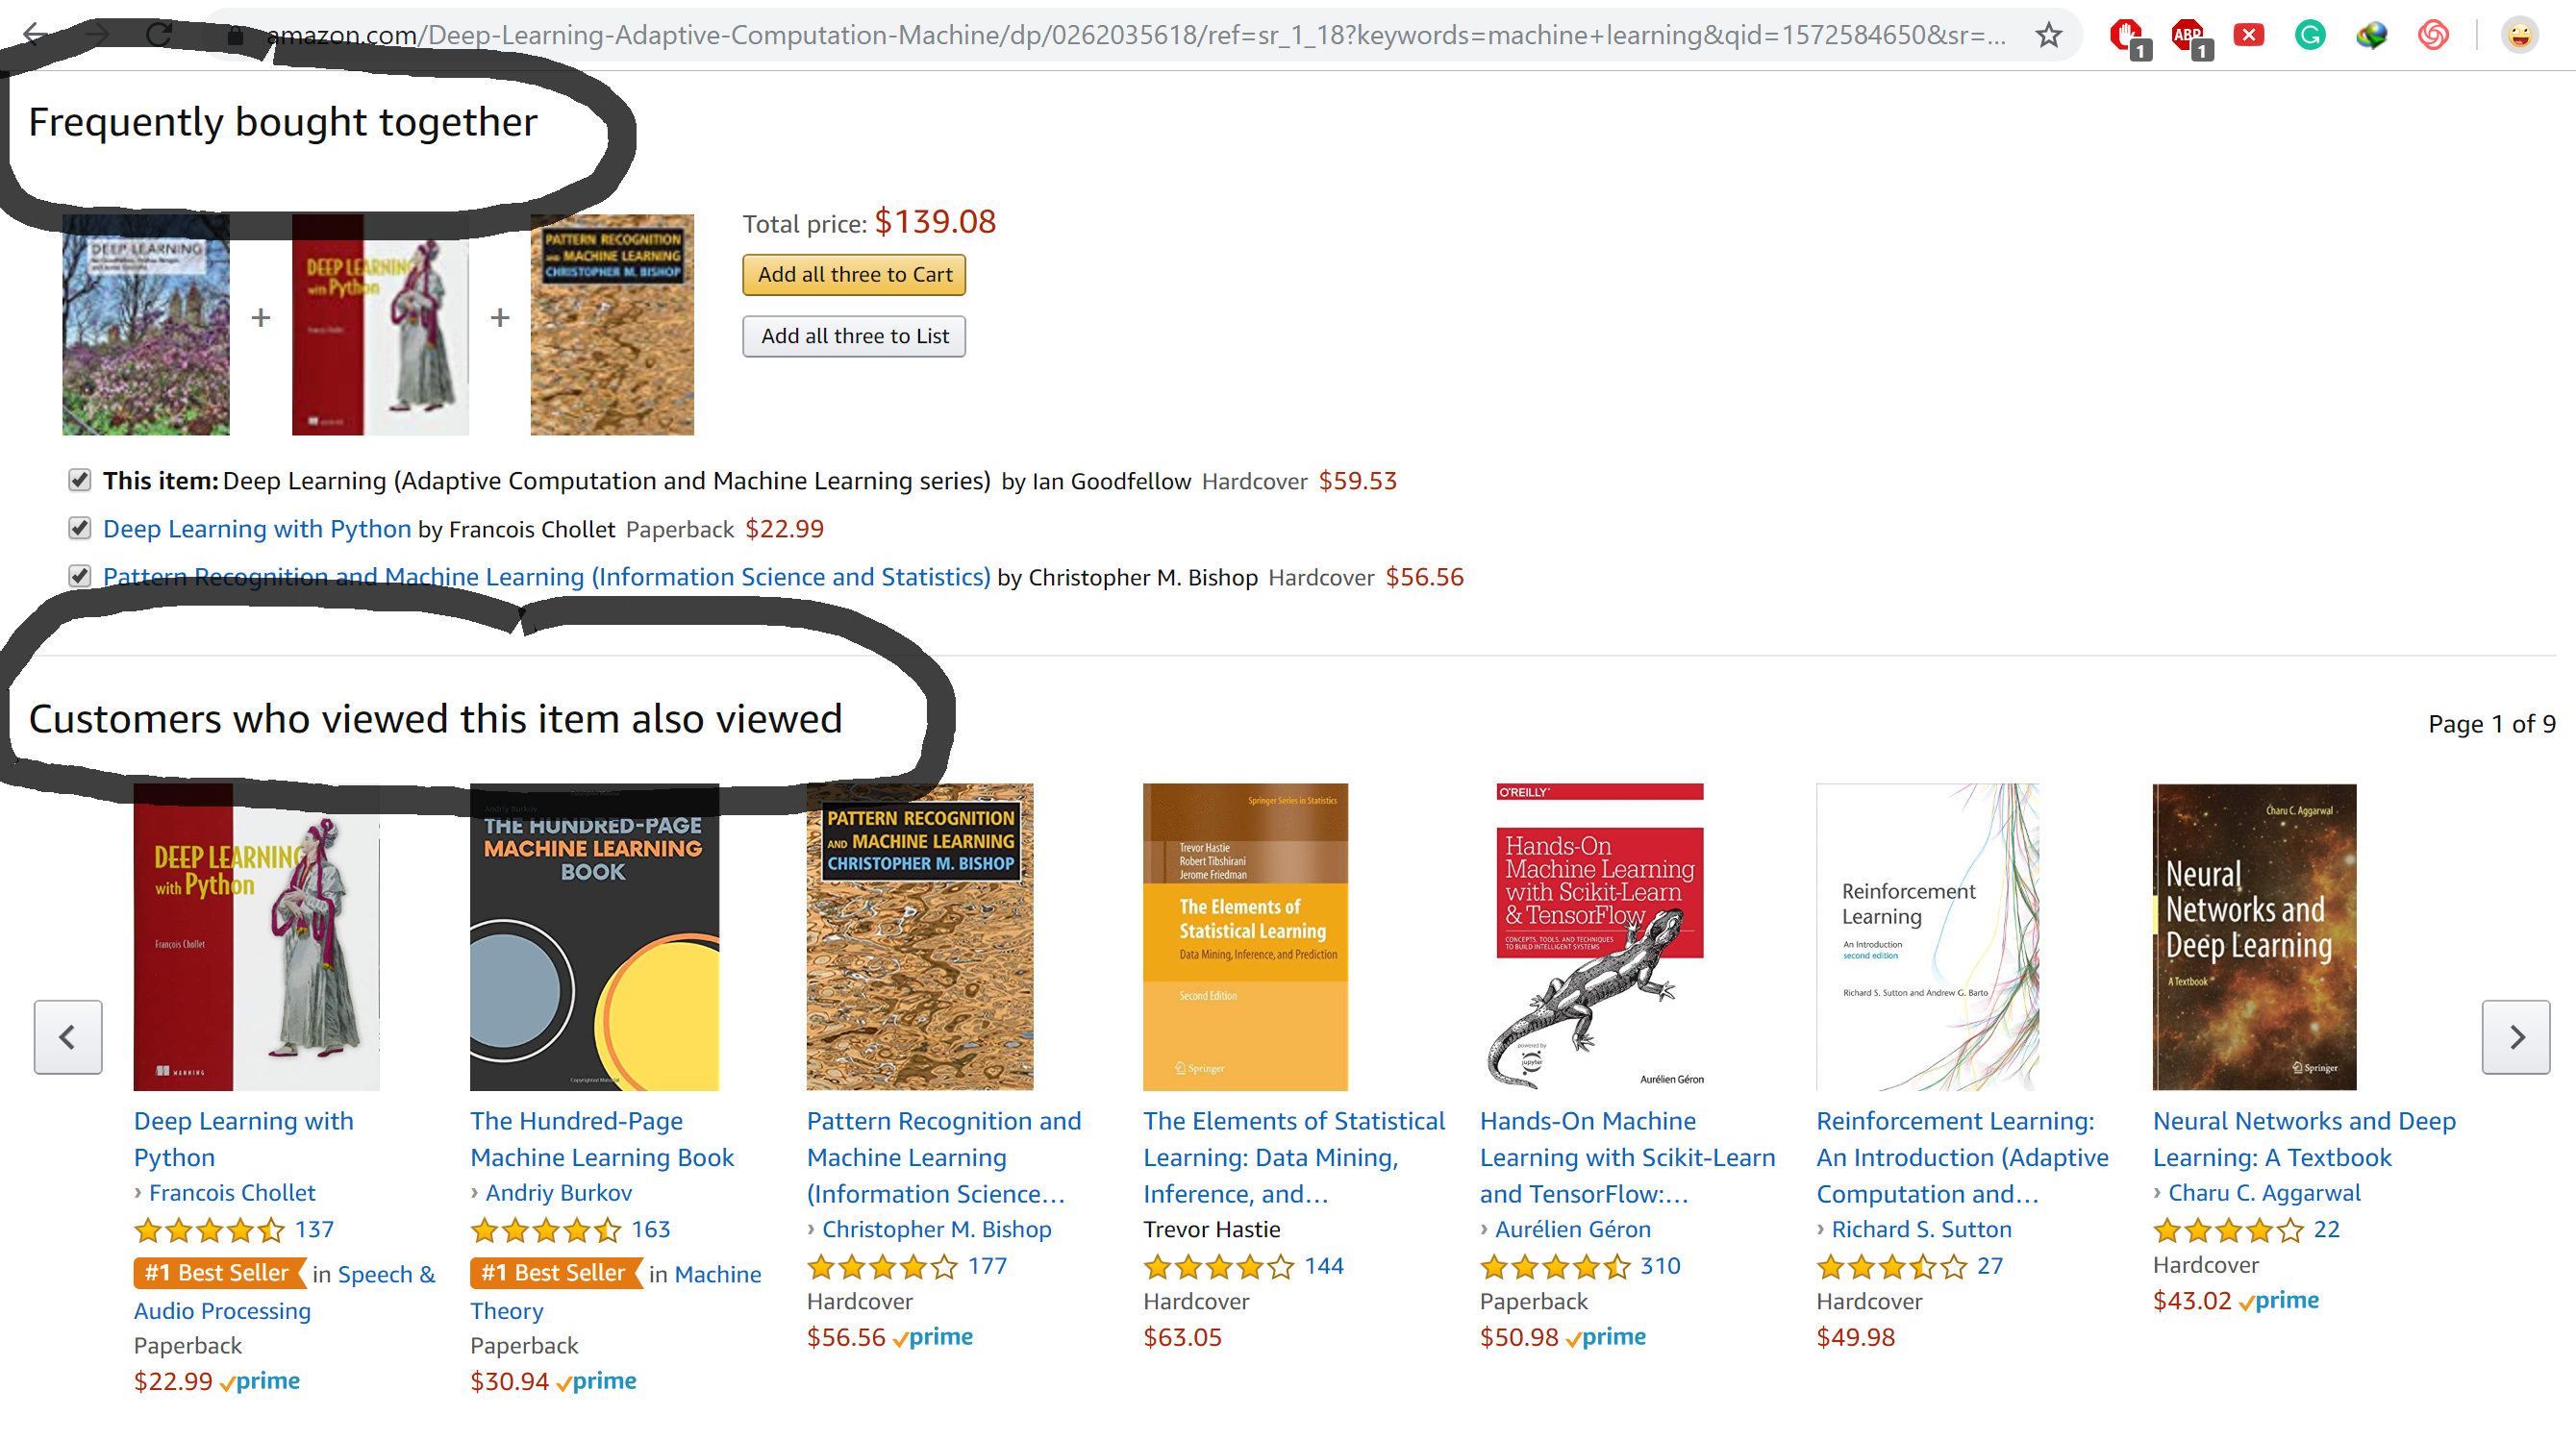
\includegraphics{images/rs1.png}

\begin{longtable}[]{@{}
  >{\raggedright\arraybackslash}p{(\columnwidth - 0\tabcolsep) * \real{0.06}}@{}}
\toprule
\begin{minipage}[b]{\linewidth}\raggedright
\#\#\# Examples - In e-commerce
\end{minipage} \\
\midrule
\endhead
\#\#\# Examples - In Social Media \\
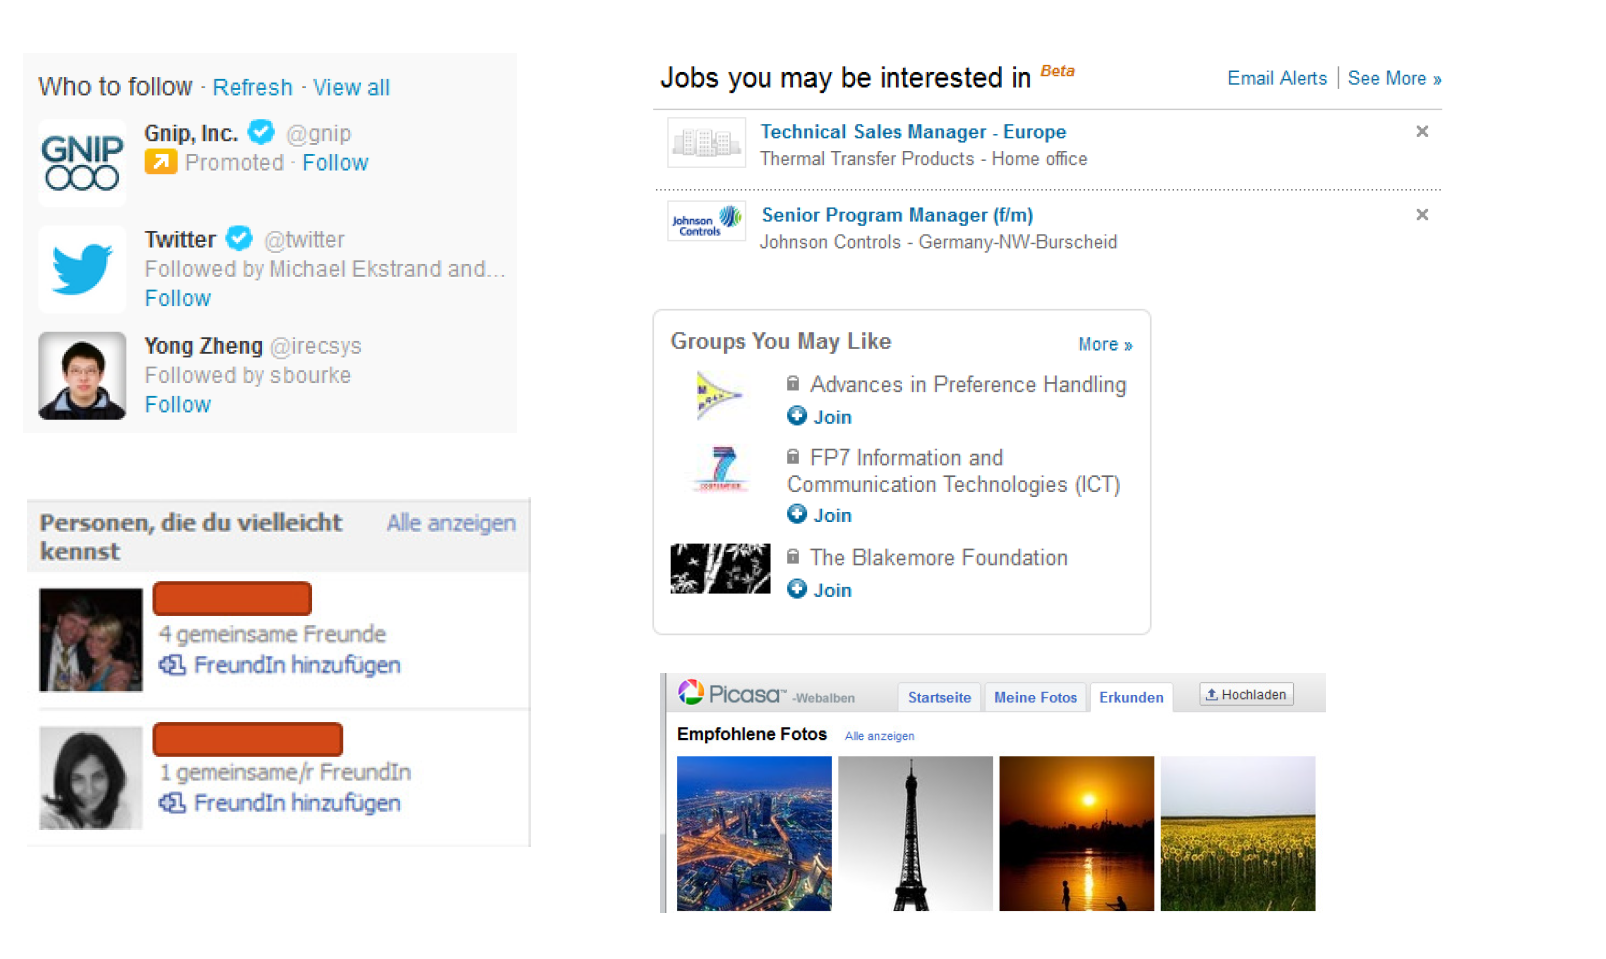
\includegraphics{images/rs3.png} \\
\bottomrule
\end{longtable}

\hypertarget{examples---mobile-apps}{%
\subsubsection{Examples - Mobile Apps}\label{examples---mobile-apps}}

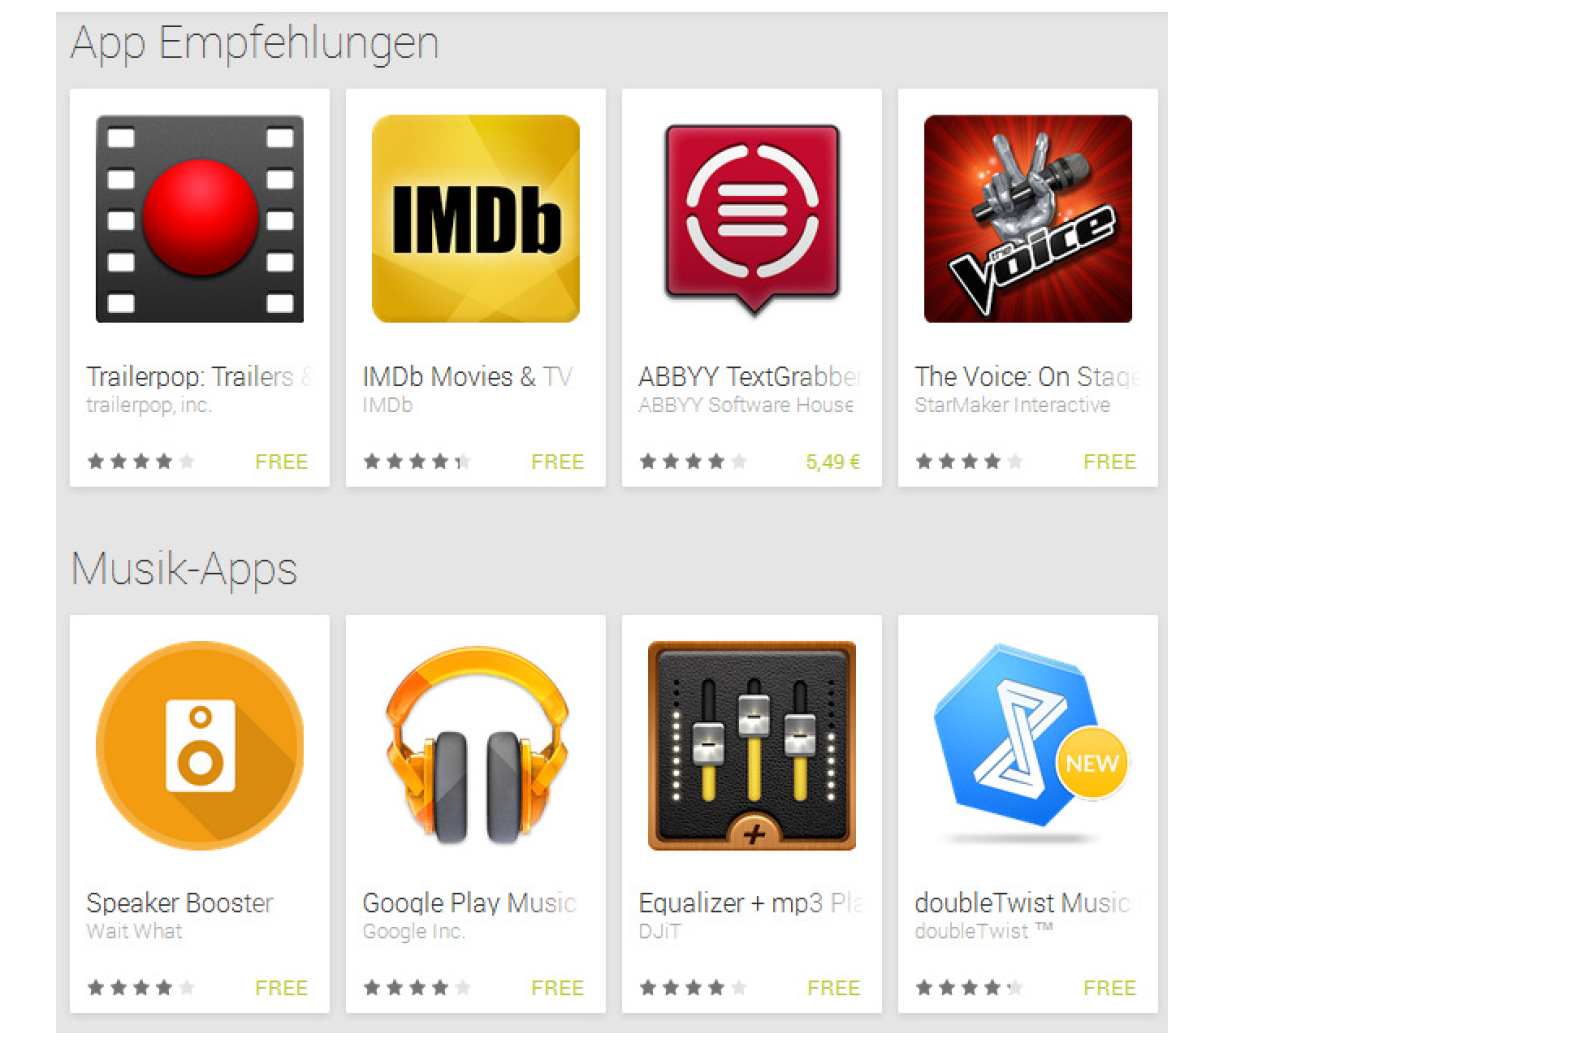
\includegraphics{images/rs4.png}

\begin{longtable}[]{@{}
  >{\raggedright\arraybackslash}p{(\columnwidth - 0\tabcolsep) * \real{0.06}}@{}}
\toprule
\begin{minipage}[b]{\linewidth}\raggedright
\#\#\# Definition - Problem domain
\end{minipage} \\
\midrule
\endhead
\#\#\# Definition - Problem domain \\
- RS are one of the \textbf{most successful and widespread applications}
of machine learning technologies in business. \\
\bottomrule
\end{longtable}

\hypertarget{two-types-of-systems}{%
\subsubsection{Two types of systems}\label{two-types-of-systems}}

\begin{itemize}
\item
  \textbf{Content- Based Filtering}: Recommeding to user A based on
  his/her existing profiles.
\item
  \textbf{Collaborative Filtering}: Recommeding to user A based on
  his/her community's profiles.
\end{itemize}

\begin{longtable}[]{@{}
  >{\raggedright\arraybackslash}p{(\columnwidth - 0\tabcolsep) * \real{0.06}}@{}}
\toprule
\begin{minipage}[b]{\linewidth}\raggedright
\#\#\# Two types of systems
\end{minipage} \\
\midrule
\endhead
\#\#\# Content- Based Filtering \\
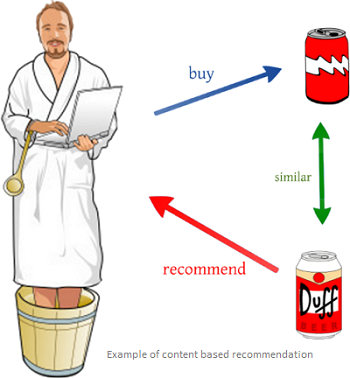
\includegraphics{images/rs5.png} \\
\bottomrule
\end{longtable}

\hypertarget{content--based-filtering}{%
\subsubsection{Content- Based
Filtering}\label{content--based-filtering}}

\begin{itemize}
\item
  Assume there are four categories of news A) Politics B) Sports C)
  Entertainment D) Technology
\item
  User A who has read 10 articles related to Technology
\item
  Recommend a new article in Technology for him to read.
\end{itemize}

\begin{longtable}[]{@{}
  >{\raggedright\arraybackslash}p{(\columnwidth - 0\tabcolsep) * \real{0.06}}@{}}
\toprule
\begin{minipage}[b]{\linewidth}\raggedright
\#\#\# Collaborative Filtering
\end{minipage} \\
\midrule
\endhead
\#\#\# Collaborative Filtering \\
- Assume there are four categories of news A) Politics B) Sports C)
Entertainment D) Technology \\
- User A who has read 10 articles related to Technology \\
- User B who has read \textbf{the same} 10 articles related to
Technology and an X article in Sports. \\
- Recommend the article X to user A. \\
\bottomrule
\end{longtable}

\hypertarget{collaborative-filtering-two-approaches}{%
\subsubsection{Collaborative Filtering: Two
approaches}\label{collaborative-filtering-two-approaches}}

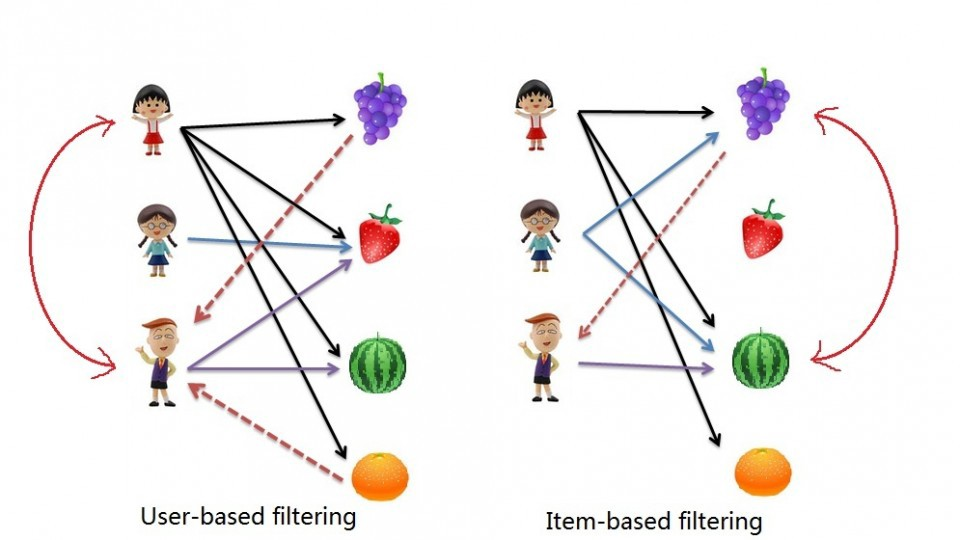
\includegraphics{images/rs7.png}

\begin{longtable}[]{@{}
  >{\raggedright\arraybackslash}p{(\columnwidth - 0\tabcolsep) * \real{0.06}}@{}}
\toprule
\begin{minipage}[b]{\linewidth}\raggedright
\#\#\# Utility Matrix
\end{minipage} \\
\midrule
\endhead
\#\#\# Nearest-neighbors (kNN) \\
- A ``pure'' CF approach and traditional baseline - Using the utility as
inputs - Returns a ranked list of items based on rating predictions \\
\bottomrule
\end{longtable}

\hypertarget{nearest-neighbors-knn}{%
\subsubsection{Nearest-neighbors (kNN)}\label{nearest-neighbors-knn}}

\begin{itemize}
\tightlist
\item
  \textbf{Assumptions}

  \begin{itemize}
  \tightlist
  \item
    If users had similar tastes in the past they will have similar
    tastes in the future
  \item
    User preferences remain stable and consistent over time
  \end{itemize}
\end{itemize}

\begin{longtable}[]{@{}
  >{\raggedright\arraybackslash}p{(\columnwidth - 0\tabcolsep) * \real{0.06}}@{}}
\toprule
\begin{minipage}[b]{\linewidth}\raggedright
\#\#\# User-based KNN
\end{minipage} \\
\midrule
\endhead
\#\#\# User-based KNN \\
\textbar{} \textbar{} Item 1\textbar{} Item 2\textbar{} Item 3\textbar{}
Item 4\textbar Item 5 \textbar{}
\textbar:------\textbar------:\textbar------:\textbar------:\textbar------:\textbar:------\textbar{}
\textbar Alice \textbar{} 5\textbar{} 3\textbar{} 4\textbar{}
4\textbar??? \textbar{} \textbar User 1 \textbar{} 3\textbar{}
1\textbar{} 2\textbar{} 3\textbar3 \textbar{} \textbar User 2 \textbar{}
4\textbar{} 3\textbar{} 4\textbar{} 3\textbar5 \textbar{} \textbar User
3 \textbar{} 3\textbar{} 3\textbar{} 1\textbar{} 4\textbar4 \textbar{}
\textbar User 4 \textbar{} 1\textbar{} 5\textbar{} 5\textbar{}
2\textbar1 \textbar{} \\
Let \(A1\) is the distance from Alice to User 1 and so on. We have: \\
\(
A1 = 3.60 \\
A2 = 1.41 \\
A3 = 3.60 \\
A4 = 5
\) \\
- For 3NN, the predicted rating of Alice for item 5 is the average of
ratings on item 5 of her 3 neast neighbors, User 1, 2 and 3. \\
- Predicted rating of Alicie on item 5 is: (3+5+4)/3 = 4. - We will
\textbf{recommend} item 5 to Alice. \\
\bottomrule
\end{longtable}

\hypertarget{item-based-knn}{%
\subsubsection{Item-based KNN}\label{item-based-knn}}

\begin{longtable}[]{@{}lrrrrl@{}}
\toprule
& Item 1 & Item 2 & Item 3 & Item 4 & Item 5 \\
\midrule
\endhead
Alice & 5 & 3 & 4 & 4 & ??? \\
User 1 & 3 & 1 & 2 & 3 & 3 \\
User 2 & 4 & 3 & 4 & 3 & 5 \\
User 3 & 3 & 3 & 1 & 4 & 4 \\
User 4 & 1 & 5 & 5 & 2 & 1 \\
\bottomrule
\end{longtable}

\begin{itemize}
\tightlist
\item
  Find the k nearest neighbors of \textbf{Item 5}.
\item
  The predicted rating of Alice on item 5 is the average rating of Alice
  on the nearest neighbors.
\end{itemize}

\begin{longtable}[]{@{}
  >{\raggedright\arraybackslash}p{(\columnwidth - 0\tabcolsep) * \real{0.06}}@{}}
\toprule
\begin{minipage}[b]{\linewidth}\raggedright
\#\#\# Item-based KNN
\end{minipage} \\
\midrule
\endhead
\#\#\# Similarity Measure \\
- Neighborhood can be decided by \textbf{similarity} measures \\
- Similarity can be measured as the inverse of the Distance \\
- The possible similarity values are between 0 and 1, where values near
to 1 indicate a strong similarity. \\
- There are many distance measure \\
- There are many similarity measure \\
\bottomrule
\end{longtable}

\hypertarget{similarity-measure}{%
\subsubsection{Similarity Measure}\label{similarity-measure}}

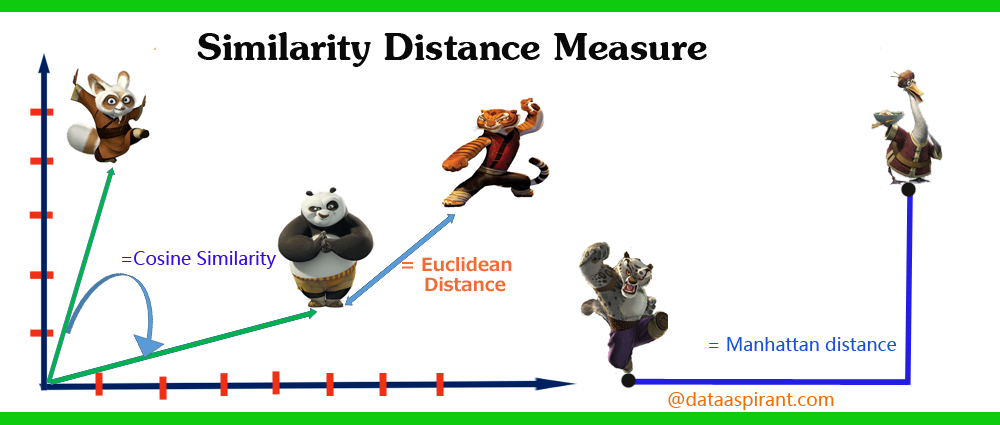
\includegraphics{images/rs9.png}

\begin{longtable}[]{@{}
  >{\raggedright\arraybackslash}p{(\columnwidth - 0\tabcolsep) * \real{0.06}}@{}}
\toprule
\begin{minipage}[b]{\linewidth}\raggedright
\#\#\# Manhattan Distance
\end{minipage} \\
\midrule
\endhead
- ManhattanDistance between Alice and User 1 (A1). \\
\textbar{} \textbar{} Item 1\textbar{} Item 2\textbar{} Item 3\textbar{}
Item 4\textbar{}
\textbar:------\textbar------:\textbar------:\textbar------:\textbar------:\textbar{}
\textbar Alice \textbar{} 5\textbar{} 3\textbar{} 4\textbar{}
4\textbar{} \textbar User 1 \textbar{} 3\textbar{} 1\textbar{}
2\textbar{} 3\textbar{} \\
\(A1  = |5-3| + |3-1|+|4-2|+|4-3| = 7\) \\
\bottomrule
\end{longtable}

\hypertarget{manhattan-vs.-euclidean}{%
\subsubsection{Manhattan vs.~Euclidean}\label{manhattan-vs.-euclidean}}

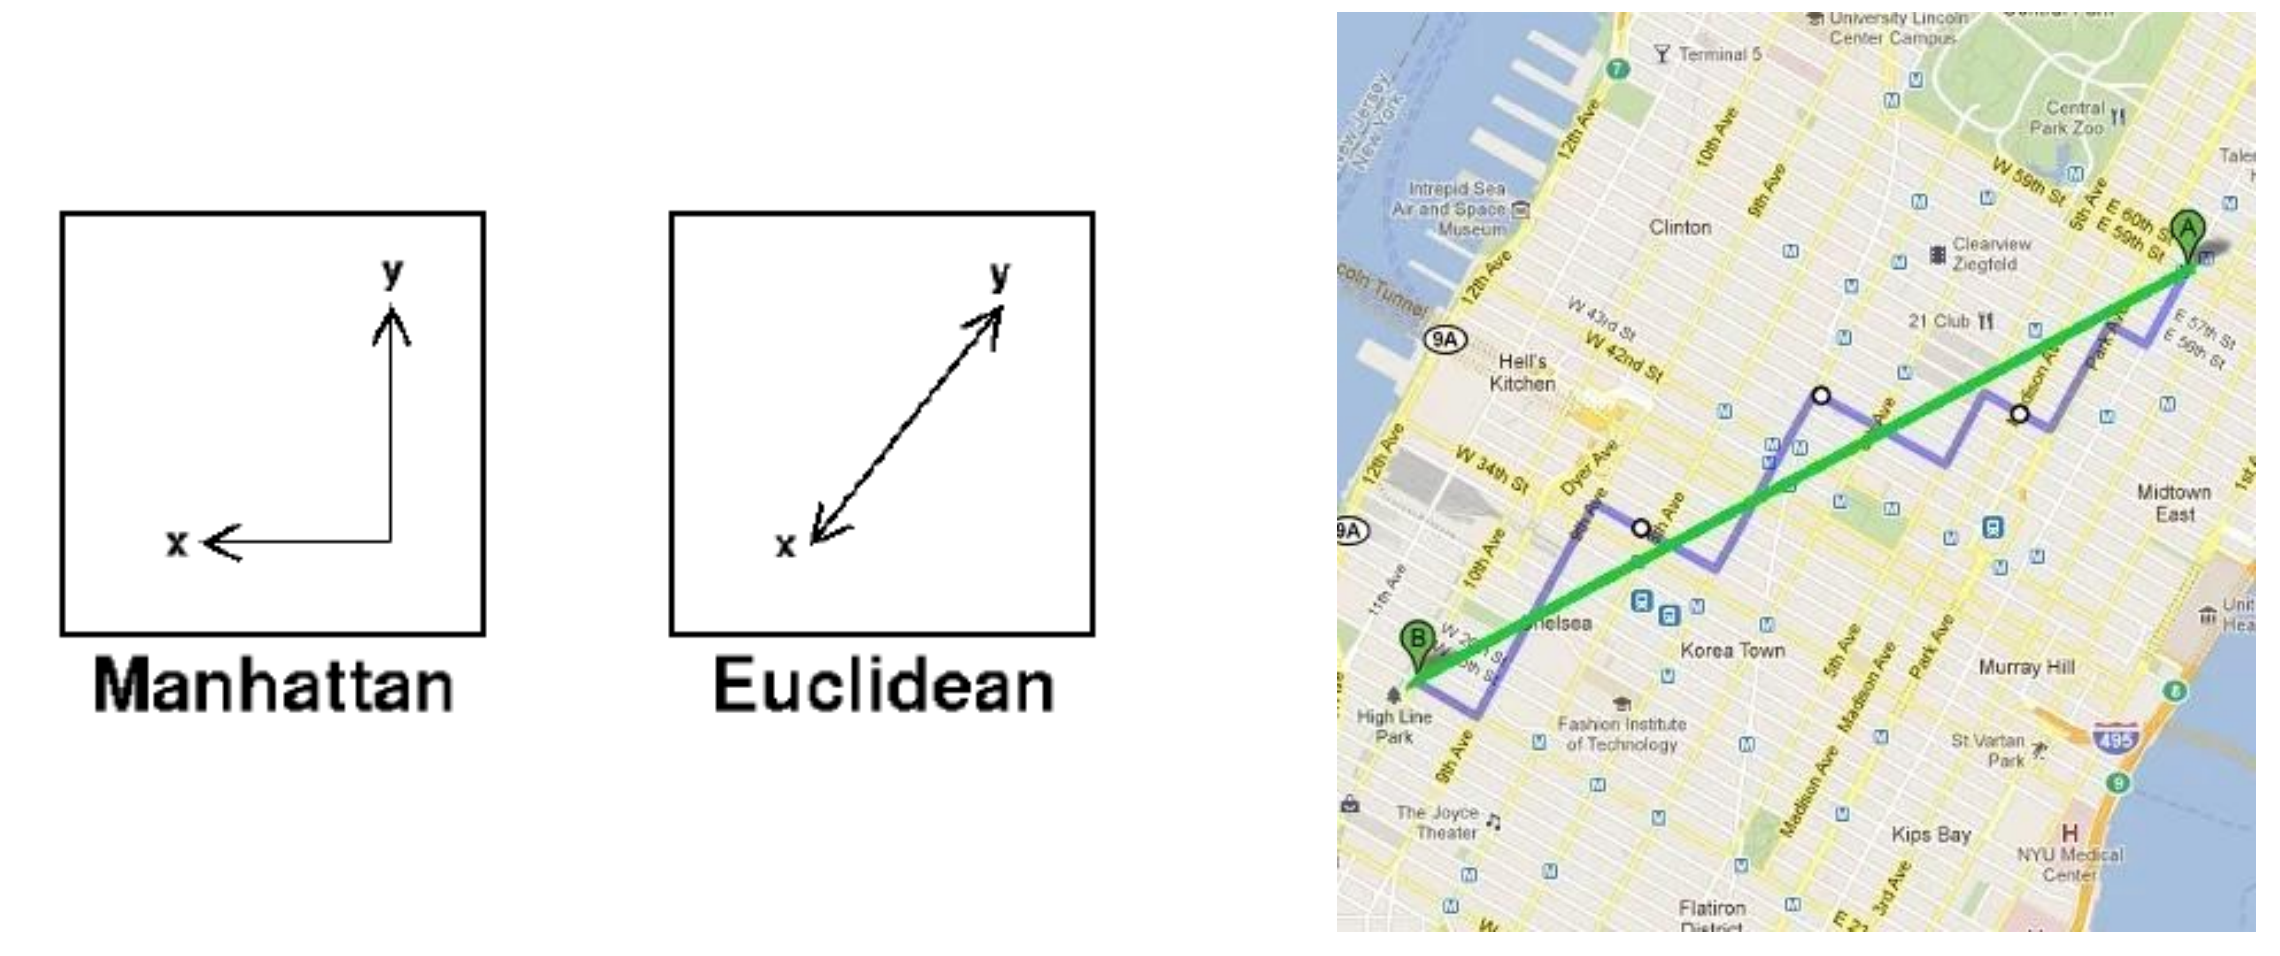
\includegraphics{images/rs11.png}

\begin{longtable}[]{@{}
  >{\raggedright\arraybackslash}p{(\columnwidth - 0\tabcolsep) * \real{0.06}}@{}}
\toprule
\begin{minipage}[b]{\linewidth}\raggedright
\#\#\# Cosine Similarity
\end{minipage} \\
\midrule
\endhead
\#\#\# Cosine Similarity Measure \\
- Cosine similarity between Alice and User 1 (S1). \\
\textbar{} \textbar{} Item 1\textbar{} Item 2\textbar{} Item 3\textbar{}
Item 4\textbar{}
\textbar:------\textbar------:\textbar------:\textbar------:\textbar------:\textbar{}
\textbar Alice \textbar{} 5\textbar{} 3\textbar{} 4\textbar{}
4\textbar{} \textbar User 1 \textbar{} 3\textbar{} 1\textbar{}
2\textbar{} 3\textbar{} \\
\(S1  = \frac{5 \cdot 3 + 3 \cdot 1 + 4 \cdot 2 + 4 \cdot 3}{\sqrt{5^2+3^2+4^2+4^2}\cdot \sqrt{3^2+1^2+2^2+3^2}} = 0.975\) \\
\bottomrule
\end{longtable}

\hypertarget{the-netflix-challenge}{%
\subsubsection{The Netflix Challenge}\label{the-netflix-challenge}}

\href{Netflix_Prize.pptx}{Link}

\end{document}
